\documentclass[tikz]{standalone} 

    \begin{document} 
     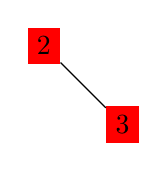
\begin{tikzpicture}[every node/.style={fill=red}, every edge/.style={draw,}] 

       % Hier stehen die Zeichen-Befehle. 
         \coordinate (x2) at (0, 0);
  \coordinate (x3) at (1, -1); 
  \node (n2) at (x2) {$2$};
  \node (n3) at (x3) {$3$}; 
  \draw (n2) edge (n3); 

        \end{tikzpicture} 
        \end{document}